%PART_3_CHAP_3_SEC_2
%WAIT a Review, ok
\clearpage
\section{Acceptabilité}\label{Exp:L_ACC}
    \subsection{Introduction}
        L’utilisabilité d’un système ne crée pas nécessairement son acceptation~\citeS{sec:acceptable}; de plus, ici nous ne traiterons pas de l'acceptabilité des kits robotiques pédagogiques à l'école en elle-même, mais de l'impact de ces kits (en l'occurrence du kit ErgoJr) sur les perceptions sociétales des individus, et donc sur l'acceptabilité de la robotique en générale, d'où le recours au questionnaire \sbg{EURO382} durant notre étude longitudinale; et au questionnaire \sht{NARS} dans une seconde étude ponctuelle.
    \subsection{Attitude toward robot (Euro382)}\label{Exp:euro}
        \paragraph{Méthode}
            Durant l'année scolaire 2016-2017, 68 élèves et 19 enseignants ont pratiqué des activités robotiques de différentes natures, et ont complété, en juin, le questionnaire \sht{EURO382}~\citeA{pdf:EURO382}. 146 élèves et 9 enseignants n'ayant pratiqué aucune activité robotique ont complété également ce questionnaire.
            Une 1\iere hypothèse est d'observer une différence entre les résultats globaux de 2012 et ceux de 2017 traduisant une acceptabilité accrue de la robotique.
            Un 2\ieme porte sur la distinction élèves, enseignants. Cette distinction pourrait avoir deux facteurs principaux: la fonction (enseignant~/~élève) ou l'âge. Pour estimer cette effet d'âge nous avons à disposition les résultats de 2012 concernant les 15-24 ans comparés au 40-54 ans.
            Une 3\ieme sur l'impact induit par la pratique d'activités robotiques. Notamment une meilleure acceptation.
            Une 4\ieme s'intéresse aux caractéristiques des activités, notamment le fait d'utiliser le livret pédagogique.
            Enfin, une 5\ieme hypothèse porte sur la distinction homme, femme, qui bien que souvent présente dans les disciplines scolaires scientifiques semble s'atténuer, voire disparaître, dans le contexte d'activités robotiques.
            \subparagraph{Population}
                En 2012 plus de 1000 personnes de chaque pays de l'union européenne ont passé ce questionnaire. Les résultats étant publiques nous pouvons les comparer avec notre échantillon constitué de $28$ enseignants et $146$ élèves de la région Nouvelle Aquitaine ayant complété ce même questionnaire (en classe \etou en ligne) durant le mois de juin 2017.
                Sur chacune des figures présentant les résultats~\citeA{pdf:euro_result} à chacune des \sht{ques} de \sht{EURO382}\citeA{pdf:EURO382}, nous pouvons repérer les modalités issues des résultats des passations de 2012, à savoir: les résultats pour la population française ($N=1059$), la population du sud-ouest ($N=120$), la population des 40-50 ans ($N=266$), la population des 15-24 ans ($N=159$), la population d'hommes français ($N=505$), la population de femmes françaises ($N=554$); toutes identifiées par~une~*. En plus de ces modalités de 2012, nous retrouvons sur nos figures l'ensemble des modalités qui ont été définies pour les besoins de notre étude. %\url{https://data.europa.eu}
                Ici, nous étudions plusieurs groupes d'individus: les enseignants et les élèves. Parmi les élèves nous nous intéressons à ceux ayant pratiqué des activités avec le kit ErgoJr ($N=68$). Ces $68$ élèves sont ensuite répartis dans différentes modalités suivant les caractéristiques des activités qu'ils ont suivi: ils peuvent avoir déclaré utiliser le livret pédagogique~\citeB{noirpoudre2016livret} fourni dans le kit ($N=13$) ou non ($N=55$); avoir utilisé d'autres kits robotiques ($N=16$); avoir pratiqué moins de 6~heures d'activités avec le robot ($N=30$), entre 6 et 25~heures ($N=22$) ou plus de 25~heures ($N=16$); avoir construit le robot ($N=12$); avoir utilisé le langage de programmation visuel \sht{snap} ($N=46$), le langage de programmation textuel \textit{Python} ($N=21$), les deux ($N=8$) ou aucun ($N=9$), il est à noter que ces deux langages sont directement accessibles via l'interface principale du robot. Les résultats présentent également les populations d'enseignants et d'élèves (ayant pratiqué ou non des activités) en fonction de leur genre, à savoir: $21$ enseignants (dont $15$ \sht{EP}), $7$ enseignantes (dont $4$ \sht{EP}), $118$ élèves garçon (dont $44$ \sht{EP}) et $96$ élèves fille (dont $24$ \sht{EP}).
        \paragraph{Résultats descriptifs}
          \subparagraph{Évolution temporelle.}
            Nous constatons des évolutions entre les passations réalisées en 2012 ($N=1059$) et nos passations de Juin 2017 ($N=242$ dont $21$ enseignants).
            De plus, les résultats régionaux (\ie Sud-ouest) de 2012 ($N=120$) sont également présentés afin d'illustrer les variations locales.
            En premier lieu, nous constatons que l'attrait pour les nouvelles technologies~\citeQ{1} est plus fort aujourd'hui, la part des \textit{très intéressé} passant de 34 à 53\prc[.]
            En revanche, sur la 2\ieme \sht{ques}, l'évolution n'est que partielle. 
            En effet, l'image du bras industriel correspond, pour le répondant, à la robotique, dans les mêmes proportions qu'en 2012 (environ 85\prc de réponses positives); alors que l'image du robot domestique humanoïde connaît une progression avec environ 75\prc en 2017 contre environ 55\prc en 2012.
                \begin{figure}[!h]
                    \begin{minipage}{0.45\linewidth}
                    \subcaption{\label{fig:QI2-1} Robot, bras industriel}
                    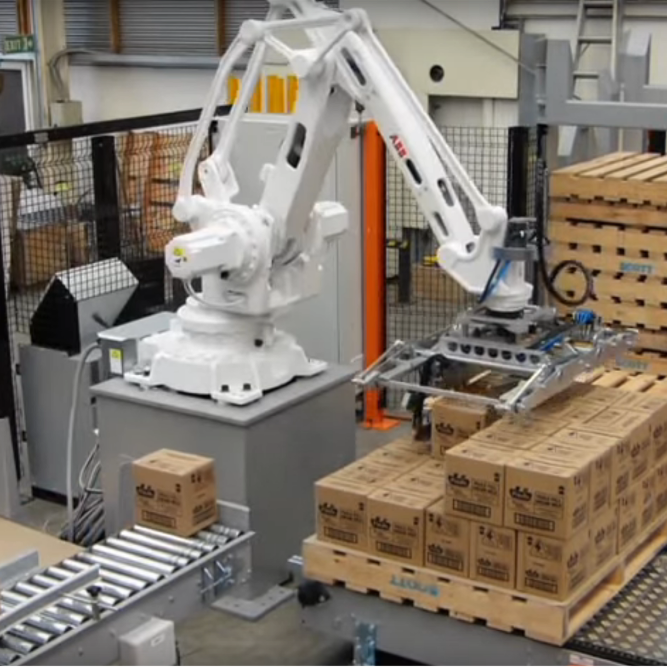
\includegraphics[width=\linewidth]{Figures/Euro-QI2_1}
                    \end{minipage}
                    \hfill
                    \begin{minipage}{0.45\linewidth}
                    \subcaption{\label{fig:QI2-2} Robot, humanoïde}
                    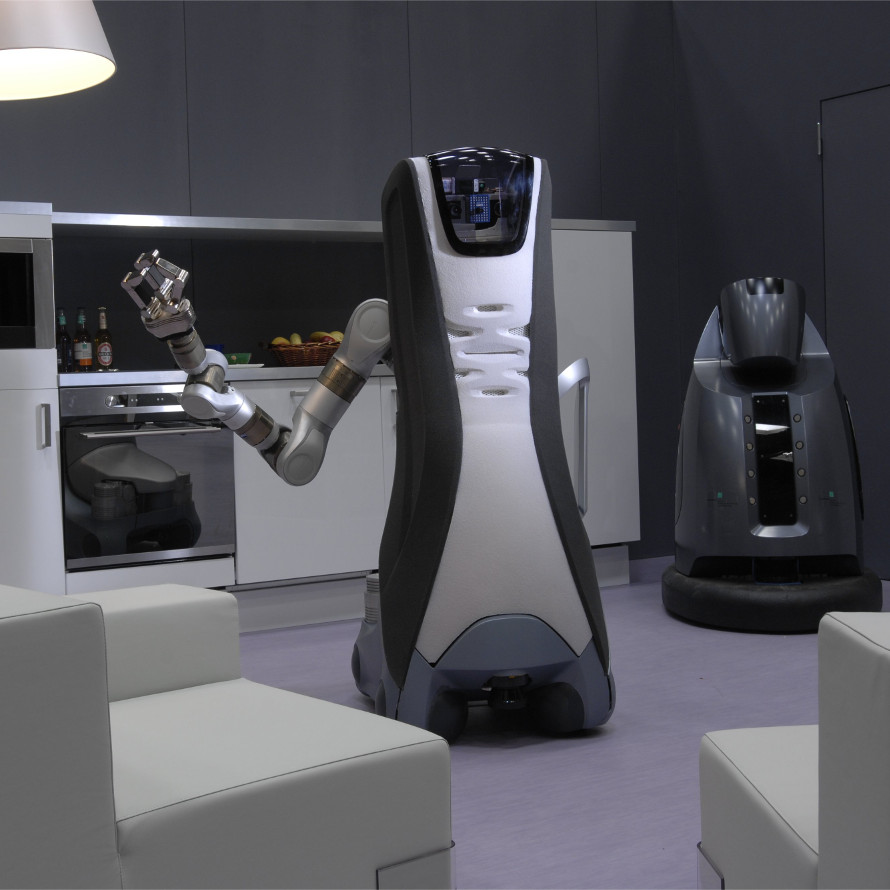
\includegraphics[width=\linewidth]{Figures/Euro-QI2_2}
                    \end{minipage}
                    \caption{Les robots visibles dans le questionnaire Euro382}
                \end{figure}
            Cependant, cette progression est à relativiser car notre échantillon, principalement constitué d'élèves (88\prc[)], obtient des scores correspondant aux 15-24 en 2012.
            La~\sht{ques}3 ({\footnotesize page~\pageref{QA3}}) montre un progression à la faveur du \textit{oui à la maison} passant de environ 10 à 25\prc et du \textit{oui~ailleurs} passant de 1 à 6\prc[.]
            Nous voyons, grâce à la~\sht{ques}4 ({\footnotesize page~\pageref{QA4}}), qu'en 5~ans, l'image que pense avoir les répondants de la robotique s'est améliorée, avec une quasi disparition de la réponse \textit{très négative}.
            Cela s'observe aussi dans la~\sht{ques}5 avec davantage d'accords sur le fait que \textit{les robots aident les gens}~\citeQ{5-1} et davantage de désaccords avec le fait que \textit{les robots volent des emplois }({\footnotesize page~\pageref{QA5-2}}).
            En revanche, il y a peu d'évolution d'opinion sur la nécessité \textit{des robots pour accomplir des tâches dangereuses ou difficiles} (massivement oui~\citeQ{5-3}), et sur \textit{la gestion prudente qu'il faut avoir vis-à-vis des robots} (massivement oui~\citeQ{5-4}). 
            Une forte évolution, concerne l'impact perçu par l'utilisation de robots sur la création d'emplois~\citeQ{5-5} qui est davantage vue comme stimulateur (avec également une forte progression des \sht{NSP} passant d'environ 10 à 20\prc[)].
            Pour la~\sht{ques}6 ({\footnotesize page~\pageref{QA6}}), nous constatons une légère progression des domaines \cro{civils} (\ie usage domestique, transport, agriculture) au dépend des activités \cro{d'État} (\ie domaine militaire, sécurité et recherche, exploration spatiale). Cependant nous retrouvons des propensions globalement identiques entre 2012 et 2017.
            En revanche, concernant la~\sht{ques}7 ({\footnotesize page~\pageref{QA7}}), nous observons une très large progression de la catégorie \cro{\textit{aucun}} (0\prc en 2012 contre 7\prc en 2017).
            Les résultats à ces deux~\sht{ques} pourraient être la traduction d'une meilleure acceptabilité de la robotique et de sa généralisation dans de nombreux usages du quotidien.
            La~\sht{ques}8, se décline en 4 sous-questions et traite de cette notion d'acceptation au quotidien pour 3 domaines: la santé, les services domestiques et le travail.
            Nous constatons un décalage entre 2012 et 2017:\textit{ se faire opérer par un robot}~\citeQ{8-1}, \textit{faire promener son chien}~\citeQ{8-2}, ou \textit{faire garder son enfant}~\citeQ{8-4} sont des situations moins inacceptables, respectivement: 13, 9, $<$2,5\prc de \textit{tout~à~fait mal~à~l'aise} en 2017 contre 38, 61 et 85\prc en 2012.
            En revanche, \textit{être assisté par un robot au travail}~\citeQ{8-3} donne des résultats plus tranchés en 2017, avec une légère majorité de réponses négatives (\ie \textit{tout~à~fait mal~à~l'aise}. 
            Nous pouvons aussi noter la disparition des catégories \textit{pas applicable} et \sht{NSP}.
            Enfin, concernant les prévisions d'une généralisation des robots domestiques~\citeQ{9}, si aucune évolution n'est relevée, un simple décalage des réponses correspondant au laps de temps entre les 2 passations (5 ans) devrait s'observer.
            Mais, moins de 2\prc estimaient en 2012 que cela était chose courante, et 12\prc que cela serait chose courante en 2017, alors qu'ils sont aujourd'hui 7\prc à considérer que cela est chose courante. Plus globalement, ils étaient environ 60\prc à estimer cette généralisation à moins de 20 ans, aujourd'hui, 5 ans après, ils sont environ 70\prc à l'estimer à moins de 10 ans. Nous constatons donc un rapprochement de l'échéance perçue par les individus sur cette~\sht{ques}.
            %%%%%%%%%%%%%%%%%%%%%%%%%%%%%%%%%%%%%%%%%%%%%%%%%%%%%%%
          \subparagraph{Distinction élèves et enseignants.}
            Afin d'illustrer l'influence de l'âge dans ces distinctions, sur  les distinctions entre les $214$ élèves et les $28$ enseignants ayant répondu, les résultats de 2012 des 40-50 ans ($N=266$) et des 15-24 ans ($N=159$) sont également présentés.
            Une première constatation est que les enseignants sont davantage intéressés par cette thématique~\citeQ{1} (75\prc de \textit{très intéressé}, contre 50\prc chez les élèves). Cependant, cet écart se retrouve aussi dans les résultats de 2012 d'où un probable effet d'âge. 
            Il en est de même pour les 2~images où l'écart ici observé est similaire à 2012 entre ces deux classes d'âges ({\footnotesize page~\pageref{QA2-1}}).
            En revanche, pour la 3\ieme \sht{ques}({\footnotesize page~\pageref{QA3}}) les tendances s'inversent: les élèves se déclarent plus utilisateurs de robots (38\prc \textit{total oui}) que ne le déclarent les enseignants (35\prc[)] notamment \textit{à~la~maison} (27\prc contre 16\prc[)], alors qu'en 2012, les plus âgés étaient ceux se déclarant le plus utilisateur (\textit{total oui}: 21\prc des 40-54 ans, contre 15\prc des 15-24 ans).
            Cette inversion s'observe également sur la~\sht{ques}4 ({\footnotesize page~\pageref{QA4}}): en 2017, les plus âgés de l'échantillon, les enseignants, qui ont un avis majoritairement pro-robot.
            Aux 5~\sht{aff} de la~\sht{ques}5, nous observons que les enseignants ont un avis qui suis la même tendance que l'évolution des réponses entre 2012 et 2017, mais avec des traits plus marqués. 
            Notamment, sur la 2\ieme \sht{aff} avec 60\prc de désaccords~\citeQ{5-2}; à l' \sht{aff}3 avec 100\prc d'accords~\citeQ{5-3}; et à l' \sht{aff} 1 et 5 avec l'absence de réponse \textit{pas~du~tout~d'accord} ({\footnotesize page~\pageref{QA5-1}~et~\pageref{QA5-5}}).
            Cependant, pour la 4\ieme \sht{aff}, seuls 86\prc des enseignants sont en accord avec la nécessité de \textit{gérer avec prudence} les robots contre 94\prc des élèves et 95\prc en 2012~\citeQ{5-4}.
            Concernant les domaines d'activités préconisés ou proscrits par les répondants pour les robots  ({\footnotesize page~\pageref{QA6}~et~\pageref{QA7}}), nous constatons des réponses similaires chez les enseignants et les élèves, comme l'étaient celles des jeunes et âgés en 2012. À noter, le recul de la préconisation du domaine militaire par les enseignants (moins de 2,5\prc contre 12\prc chez les élèves et 14\prc en 2012).
            Comme pour la 5\ieme \sht{ques}, les enseignants suivent une tendance identique à celle des élèves: une meilleure acceptation de la robotique ({\footnotesize page~\pageref{QA8-1},~\pageref{QA8-2}~et~\pageref{QA8-4}}), avec 2 nuances: sur la 3\ieme \sht{aff}, 54\prc de \textit{tout~à~fait mal~à~l'aise} contre 26\prc chez les élèves et 13\prc en 2012 ({\footnotesize page~\pageref{QA8-3}}); et sur la 1\iere \sht{aff}, la distinction entre enseignants et élèves de 2017 s'inverse par rapport à celle observée entre les 40-54 et les 15-24 ans en 2012: les jeunes étaient davantage \textit{mal~à~l'aise}, aujourd'hui ce sont les enseignants.
            En outre, à la 3\ieme \sht{aff}, nous voyons apparaître une distinction entre élèves et enseignants, là où en 2012 les résultats des 14-25 ans et des 40-54 ans étaient similaires.
            Enfin, à la~\sht{ques}9 ({\footnotesize page~\pageref{QA9}}), une même évolution est constatée entre élèves et enseignants mais plus exacerbée: 79\prc des enseignants estimaient que les robots domestiques seront \textit{une chose courante dans 10 ans ou moins} contre 66\prc des élèves. Mais surtout, ils sont 0\prc à l'estimer \textit{dans plus de 20 ans} (contre 8\prc des élèves).
            %%%%%%%%%%%%%%%%%%%%%%%%%%%%%%%%%%%%%%%%%%%%%%%%%%%%%%%
          \subparagraph{Distinction avec et sans activité robotique.}
            Des distinctions entre les réponses des $68$ \sht{EP} et celles des $146$ \sht{ENP}.
            En effet, dès la 1\iere \sht{ques}({\footnotesize page~\pageref{QA1}}), nous observons qu'aucun des \sht{EP} se déclare \textit{pas du tout intéressé} par les nouvelles technologies contre 4\prc des \sht{ENP}, et qu'ils ont un intérêt déclaré supérieur (57 contre 47\prc[)]. 
            %nous pouvons noter que seules les étudiantes \sht{ENP} obtiennent un score plutôt faible 31\prc mais comparable à ceux obtenus en moyenne en 2012.
            Pour la 1\iere image~\citeF{fig:QI2-1} pas de différence entre les \sht{EP} et les \sht{ENP}. 
            En revanche, pour la 2\nde avec le robot humanoïde~\citeF{fig:QI2-2}, nous voyons une progression des \sht{NSP} chez les \sht{EP} (13\prc[)] et pas chez les \sht{ENP} (2\prc[)].
            La 3\ieme \sht{ques}({\footnotesize page~\pageref{QA3}}) montre de légères différences là où nous aurions attendu avoir une forte distinction:
            la principale concerne la propension de ceux ayant répondu \textit{oui~à~la~maison} étant de 30\prc chez les \sht{ENP} contre 19\prc chez les \sht{EP}, cet écart est au profit du \textit{oui ailleurs} étant de 3\prc chez les \sht{ENP} contre 14\prc chez les \sht{EP}, soit 36\prc \textit{oui} tout confondu pour les \sht{ENP} et 38\prc pour les \sht{EP}.
            À noter aussi, une plus forte présence du \sht{NSP} pour les \sht{EP}: 7\prc contre 2\prc[.]
            À la~\sht{ques}4 ({\footnotesize page~\pageref{QA4}}), nous observons que les \sht{EP} ont un \textit{à priori} que les \sht{ENP} n'ont pas (moins de 2\prc d'avis négatifs contre 14\prc des \sht{ENP}).
            À la 1\iere \sht{aff}({\footnotesize page~\pageref{QA5-1}}), nous constatons que environ 90\prc des élèves s'accordent à dire que \textit{les robots sont une bonne chose pour la société} mais de manière moins radicale chez les \sht{ENP}: 20\prc de \textit{Tout~à~fait~d'accord} contre 37\prc chez les \sht{ENP}.
            À l'inverse, sur la 2\ieme \sht{aff}({\footnotesize page~\pageref{QA5-2}}) la radicalité s'observe chez les \sht{EP}: environ 45\prc des élèves sont en désaccord avec l'idée que \textit{les robots volent les emplois} et seuls 10\prc des \sht{ENP} ne sont \textit{pas~du~tout~d'accord}, contre 21\prc des \sht{EP}.
            Concernant \textit{la nécessité des robots pour les taĉhes dangereuses}~\citeQ{5-3}, nous notons une propension légèrement supérieure d'accords chez les \sht{EP} (89\prc contre 86\prc[)] et l'apparition de la réponse \sht{NSP} à hauteur de 3\prc contre 0\prc[)].
            Pour \textit{la gestion prudente de cette technologie}~\citeQ{5-4} c'est pour les \sht{ENP} que nous constatons un accord légèrement supérieur: 95\prc contre 94\prc[.]
            Concernant la \textit{stimulation de la création d'emploi}~\citeQ{5-5}, nous observons une plus nette distinction, les \sht{EP} étant majoritairement en accord (56\prc[)] ce qui n'est pas le cas chez les \sht{ENP}: 41\prc d'accord. Nous constatons également chez ces 2 groupes une forte présence de la réponse \sht{NSP} (environ 21\prc[)].
            Au niveau des domaines d'activités préconisées et à proscrire ({\footnotesize page~\pageref{QA6}~et~\pageref{QA7}}), les \sht{EP} et les \sht{ENP} ont des résultats globalement identiques, sauf pour le domaine à proscrire \cro{\textit{aucun}} où les \sht{EP} semblent plus proches des enseignants que des \sht{ENP}: respectivement 9, 11 et 5\prc[.]
            Globalement, sur les aspects abordés dans les~\sht{ques} de la 8\ieme \sht{ques}, nous pouvons noter un ressenti légèrement plus positif côté \sht{EP}, avec des réponses égales à 9 \etou 10 (0 = \textit{tout~à~fait mal~à~l'aise} et 10 = \textit{tout~à~fait à~l'aise}) plus fréquentes pour ces 4~\sht{ques}({\footnotesize page~\pageref{QA8-1},~\pageref{QA8-2},~\pageref{QA8-3}~et~\pageref{QA8-4}}). 
            Cet aspect pourrait montrer l'impact de la pratique d'activités pédagogiques sur l'acceptabilité de la robotique. De plus, la présence accrue de réponses \sht{NSP} pourrait traduire une prise de conscience chez les \sht{EP} d'une vision plus complexe de la robotique.
            Sur les perspectives de \textit{généralisation de la robotique domestique} les \sht{EP} semblent être plus précis: 46\prc l'estiment à \textit{10 ans}, les \sht{ENP} semblant plus indécis (résultats plus distribués). Pour ces 2 groupes, environ 8\prc pensent que \textit{c'est déjà une chose courante} et 4\prc ne se prononcent pas.
            %%%%%%%%%%%%%%%%%%%%%%%%%%%%%%%%%%%%%%%%%%%%%%%%%%%%%%%
          \subparagraph{Distinction entre les caractéristiques des activités.}
            Nous constatons des distinctions issues des caractéristiques des activités proposées par les enseignants aux $68$ élèves ayant complété le questionnaire. 
            Cependant, même si ces modalités ont révélé avoir un impact, celui-ci reste localisé; aucune des modalités n'offrant de distinction significative sur l'ensemble des~\sht{ques} du questionnaire.
            Concernant la 1\iere \sht{ques}({\footnotesize page~\pageref{QA1}}), nous constatons que les élèves n'ayant pas utilisé les langages de programmation par défaut (\sht{snap} et \textit{Python}) ont un score bien inférieur aux autres (11\prc[)] et que les élèves \sht{ENP} avec \sht{snap} ont également un score faible 36\prc comparé à la moyenne de notre échantillon 53\prc[.]
            Pour la 2\ieme, c'est la modalité \textit{utilise un autre kit} qui offre une distinction notamment pour la 1\iere image~\citeF{fig:QI2-1} correspondant davantage à la représentation de robot pour eux (44\prc contre 19\prc en moye nne).
            Sur la 2\nde~image~\citeF{fig:QI2-2} on note la forte présence des réponses \sht{NSP} dans certaines modalités (13\prc en moyenne avec des pics allant jusqu'à 21\prc[)], mais aussi son absence dans les modalités \textit{avec livret} et \textit{utilise \sht{snap} et python}.
            Sur la~\sht{ques}3 ({\footnotesize page~\pageref{QA3}}), un ensemble de facteurs semble déterminer l'apparition de la réponse \sht{NSP}: le fait d'avoir utilisé le livret pédagogique, d'avoir construit le robot, d'avoir utilisé le langage de programmation textuel \textit{Python} et d'avoir plus de 25h de pratique, fait tendre les \sht{NSP} vers 0. À noter également, que les répondants des modalités \textit{utilisent d'autres kits} et \textit{plus de 25h de pratique} ont un taux de \textit{oui} plus élevé (environ 50\prc[)] que la moyenne des \sht{EP} (38\prc[)].
            Sur les \textit{à priori}~\citeQ{4}, ils sont plutôt \textit{très positifs} pour la modalité \textit{avec livret} et \textit{utilise \sht{snap} et Python} (46 et 62\prc contre 28\prc en moyenne), avec une niche de réponses \textit{plutôt négatif} dans la modalité \textit{n'utilise ni \sht{snap}, ni Python} (11\prc contre moins de 2,5\prc en moyenne).
            À la 1\iere \sht{aff} de la~\sht{ques}5 ({\footnotesize page~\pageref{QA5-1}}), la modalité \textit{avec livret} se démarque avec 62\prc d'accord contre 37\prc en moyenne. L'absence de désaccord pour les modalités \textit{utilise Python} et \textit{entre 6 et 25h de pratique} est aussi à noter.
            À la 2\ieme \sht{aff}({\footnotesize page~\pageref{QA5-2}}), ici encore c'est la modalité \textit{avec livret} qui totalise l'accord le plus grand (31\prc contre 12\prc en moyenne), mais aussi le désaccord le plus grand (38\prc contre 21\prc[)] ex~aequo avec la modalité \textit{utilise \sht{snap} et Python} qui, de plus, est la 2\nde~modalité où la réponse \sht{NSP} est la plus présente (12\prc contre 4\prc[)] et la seule marquée par l'absence de réponse \textit{tout~à~fait~d'accord}.
            À la 3\ieme \sht{aff}({\footnotesize page~\pageref{QA5-3}}), nous retrouvons une majorité d'accords et une absence de désaccords pour les modalités \textit{avec livret} et \textit{utilise \sht{snap} et Python} (69 et 88\prc contre 57\prc en moyenne). Nous notons aussi, une forte présence des \sht{NSP} dans la modalité \textit{ni \sht{snap}, ni Python} (11\prc contre 3\prc[)].
            À la 4\ieme \sht{aff}({\footnotesize page~\pageref{QA5-4}}), une nouvelle fois, c'est la modalité \textit{à construit le robot} qui totalise le plus de réponses \sht{NSP} (9\prc contre moins de 2,5\prc[)] et la modalité \textit{utilise \sht{snap} et Python} pour la réponse \textit{tout~à~fait~d'accord} (75\prc contre 49\prc[)].
            Le maximum de désaccords est atteint par la modalité \textit{à construit le robot} avec 17\prc de \textit{plutôt~pas~d'accord} talonné par la modalité \textit{avec livret} à 15\prc[.]
            À la 5\ieme \sht{aff}({\footnotesize page~\pageref{QA5-5}}), nous constatons que les modalités \textit{utilise \sht{snap} et Python} et \textit{n'utilise ni \sht{snap}, ni Python} sont les seules à ne totaliser aucune réponse \sht{NSP} là où toutes les autres avoisinent les 20\prc[.] À noter également, l'absence de désaccords pour les 4 modalités \textit{avec livret, plus de 25h de pratique, à construit le robot} et \textit{utilise \sht{snap} et Python} contre 7\prc en moyenne. Cette dernière modalité est ici encore la modalité totalisant le plus de réponses \textit{tout~à~fait d'accord} (50\prc contre 18\prc en moyenne).
            Concernant les domaines d'activités préconisés et à proscrire ({\footnotesize page~\pageref{QA6}~et~\pageref{QA7}}), le nombre de réponses possibles (3 parmi 12 soit 220 possibilités) associé à un effectif relativement faible dans certaines modalités ($Min=8$) ne permet pas la mise en évidence de variations suffisamment importantes.
            Au niveau du ressenti abordé en~\sht{ques}8, nous constatons à la 1\iere \sht{aff}({\footnotesize page~\pageref{QA8-1}}) que, là encore, les modalités \textit{avec livret} et \textit{utilise \sht{snap} et Python} offrent les réponses les plus saillantes: cette 1\iere modalité montrant une meilleure acceptation (38\prc de réponses supérieures à 8 points, contre 18\prc en moyenne); à l'inverse, la 2\nde, montre une acceptation plus faible (63\prc de réponses inférieures à 3, contre 34\prc[)].
            À la 2\ieme \sht{aff}({\footnotesize page~\pageref{QA8-2}}), nous notons principalement le total des réponses supérieures à 7 atteignant 42\prc dans la modalité \textit{a construit le robot} contre 17\prc en moyenne.
            À la 3\ieme \sht{aff}({\footnotesize page~\pageref{QA8-3}}), nous constatons que les scores (\textit{tout~à~fait mal~à~l'aise}) pour les modalités \textit{avec livret, à construit le robot} et \textit{utilise \sht{snap} et Python} sont plus similaires à ceux des enseignants qu'à ceux des autres élèves, respectivement: 46, 33, 50\prc pour ces 3~modalités, 54\prc pour les enseignants, 26\prc pour les élèves contre 13\prc en 2012.
            À la 4\ieme \sht{aff}({\footnotesize page~\pageref{QA8-4}}), c'est encore la modalité \textit{a construit le robot} qui montre la plus grande acceptation de la robotique (33\prc de réponses supérieures à 7, contre 16\prc en moyenne).
            Enfin, la 9\ieme \sht{ques}({\footnotesize page~\pageref{QA9}}) montre une nette différence pour la modalité \textit{avec livret} où \textit{la généralisation de la robotique dans les tâches ménagères} n'est pas envisagée avant \textit{20 ans ou plus} pour 61\prc[,] contre 25\prc en moyenne. Une tendance similaire pour la modalité \textit{a construit le robot} est observée (42\prc[)], nous notons aussi une forte présence de la réponse \textit{jamais} pour cette 1\iere modalité (8\prc contre moins de 2,5\prc en moyenne) et pour la modalité \textit{utilise d'autres kits} (6\prc[)] à laquelle s'ajoute une absence de réponse \sht{NSP}, également absente dans la modalité \textit{a construit le robot}.
            %%%%%%%%%%%%%%%%%%%%%%%%%%%%%%%%%%%%%%%%%%%%%%%%%%%%%%%
          \subparagraph{Distinction homme et femme.}
            Afin d'illustrer l'influence du sexe dans les distinctions entre les enseignants ($N=21$) et les enseignantes ($N=7$) et entre les $118$ garçons (dont $44$ \sht{EP}) et les $98$ filles (dont $24$ \sht{EP}), les résultats des françaises en 2012 ($N=554$) et des français ($N=505$) sont également présentés.
            Deux premiers constats sur la 1\iere \sht{ques}({\footnotesize page~\pageref{QA1}}): les garçons \sht{EP} ou \sht{ENP} sont relativement identiques, tandis que chez les filles on observe un intérêt accru pour les sciences pour celles ayant participé à des activités robotiques: 50\prc contre 31\prc des filles \sht{ENP}.
            D'autre part, nous notons que les enseignantes ont un intérêt plus faible que leurs élèves (43\prc contre 50\prc chez les filles et 61\prc chez les garçons), à l'inverse les enseignants ont un intérêt bien supérieur aux autres (86\prc[)]. Dans tous les cas, nous observons une progression positive en comparaison des résultats \textit{homme / femme} de 2012.
            En revanche, à la 2\ieme \sht{ques}, 1\iere image~\citeF{QA2-1}, chez les filles, nous notons un recul (21\prc contre 35\prc en 2012) au profit du \sht{NSP} pour le \sht{EP} (12\prc[)] et de la réponse \textit{correspond plutôt~mal} pour les \sht{ENP} (19\prc[)]. 
            Cependant, chez les enseignantes, nous observons le phénomène inverse avec une diminution de la réponse \textit{plutôt~bien} au profit de la réponse \textit{très~bien}.
            Chez les hommes, nous observons une progression par rapport à 2012, mais plus forte pour les enseignants et les garçons \sht{EP} que pour les garçons \sht{ENP} (respectivement: 37, 57, 48 et 41\prc[)]. 
            Pour la 2\nde~image~\citeF{QA2-2}, nous observons un recul pour les enseignantes en comparaison des résultats féminins de 2012 (14\prc contre 27\prc[)] et une avancée pour les filles (environ 43\prc[)]. 
            De plus, nous observons, comme sur l'image précédente, qu'il y a chez celles \sht{EP}, une absence des réponses \textit{plutôt~mal} et \textit{très~mal}, ainsi qu'une forte présence de \sht{NSP} (21\prc[)].\par% 
            Côté garçons, nous observons une avancée pour les \sht{EP} et les enseignants, mais pas pour les \sht{ENP} en comparaison de 2012 (respectivement 41, 33, 28 et 28\prc[)].
            Ces réponses soulignent l'impact différent qu'ont eu les activités sur les filles et les garçons.
            Concernant la proximité d'utilisation~\citeQ{3}, nous observons une forte croissance des réponses oui (environ 45\prc chez les femmes et 30\prc chez les hommes, contre environ 10 et 20\prc en 2012). 
            Ceci s'observe particulièrement sur le \textit{oui~à~la~maison} chez les élèves (fille ou garçon) \sht{ENP}.
            Par ailleurs, chez les filles \sht{EP}, une forte augmentation des \sht{NSP} est encore constatée (11\prc contre moins de 4\prc pour les autres groupes).
            Concernant leur \textit{à priori}~\citeQ{4}, nous notons que chez les enseignants et les \sht{EP}, il y a une absence de réponse \textit{très~négative} et ceci indépendemment du sexe des individus.
            Cependant, les hommes ont plus de réponses \textit{très~positive} de 30\prc contre 10\prc chez les filles. 
            En outre, nous constatons que pour les filles \sht{ENP} les scores sont comparables à ceux de 2012 (6\prc contre 5\prc[)].
            À la 1\iere \sht{aff} de la~\sht{ques}5 ({\footnotesize page~\pageref{QA5-1}}) la part de réponses \textit{pas~du~tout~d'accord} dans la moyenne des résultats est exclusivement portée par les garçons \sht{ENP}.
            Nous constatons également que les filles \sht{EP} ont des résultats plus proches des hommes \sht{ENP}, et que les filles \sht{ENP} conservent des résultats semblables à ceux de 2012. 
            Notons, chez les hommes, qu'aucun enseignant n'a répondu en désaccord, et que la part de réponses \textit{tout~à~fait~d'accord} chez les garçons \sht{EP} est bien plus importante (45\prc contre de 11 à 29\prc[)].
            À la 2\ieme \sht{aff}({\footnotesize page~\pageref{QA5-2}}), nous voyons une très nette évolution vers le désaccord avec quelques spécificités: une forte présence de la réponse \sht{NSP} chez les enseignants (14\prc[)], associée à une absence de la réponse \textit{tout~à~fait~d'accord} et un effet de la pratique des activités comme accentuateur chez les garçons (57\prc de désaccords contre 47\prc des \sht{ENP}) et comme atténuateur chez les filles (16\prc de désaccords contre 29\prc des \sht{ENP}).
            À l' \sht{aff} suivante~\citeQ{5-3}, nous observons le même effet accentuateur chez les garçons (68\prc de \textit{tout~à~fait~d'accord} contre 51\prc des \sht{ENP} et 52\prc en 2012) et atténuateur chez les filles (47\prc de \textit{tout~à~fait~d'accord} contre 38\prc des \sht{ENP} et 40\prc en 2012).
            Les enseignant(e)s sont à 100\prc en accord avec cette~\sht{ques}, avec un peu plus d'intensité chez les enseignantes (71\prc contre 62\prc chez les enseignants).
            La 4\ieme \sht{aff}({\footnotesize page~\pageref{QA5-4}}) montre qu'être enseignant(e)s ou avoir pratiqué des activités robotiques rend davantage en désaccord avec la prudence que nécessite cette technologie, tandis que les \sht{ENP} ont un niveau d'accord supérieur à celui constaté en 2012. Cet écart est d'autant plus visible chez les femmes.
            Pour la 5\ieme \sht{aff}({\footnotesize page~\pageref{QA5-5}}), nous constatons une augmentation de l'accord chez les enseignants, mais plus marquée chez les hommes (86\prc contre 39\prc en 2012 chez les hommes, et 57\prc contre 31\prc en 2012 chez les femmes). 
            Pour cette~\sht{ques}, nous constatons, là encore, un impact différent de la pratique des activités en fonction du sexe de l'élève, à savoir: un \sht{NSP} massif chez les filles \sht{EP} et chez les garçons \sht{ENP} (33 et 26\prc[)]; un accord plus fort chez les garçons \sht{EP} et chez les filles \sht{ENP} (70 et 37\prc[)]; réciproquement, un désaccord plus fort chez les garçons \sht{ENP} et chez les filles \sht{EP} (28 et 37\prc[)].
            Pour les domaines d'activités à préconiser en~\sht{ques}6 ({\footnotesize page~\pageref{QA6}}), nous notons très peu de variations. Cependant, chez les enseignantes il y a une absence de réponse dans le domaine \textit{des soins de santé}.
            De plus, à la~\sht{ques}7 ({\footnotesize page~\pageref{QA7}}), c'est ce domaine qui est majoritaire chez les enseignants (29\prc[)]. 
            En revanche, le domaine militaire n'apparaît pas dans leurs domaines proscrits. 
            Pour les autres groupes et autres domaines, nous observons une distribution plutôt homogène et similaire à celle de 2012.
            Aux~\sht{ques}1, 2 et 4, de la~\sht{ques}8 ({\footnotesize page~\pageref{QA8-1},~\pageref{QA8-2}~et~\pageref{QA8-4}}), nous ne constatons aucune variation notable.
            En revanche, à l' \sht{aff}3 ({\footnotesize page~\pageref{QA8-3}}), il y a une accentuation du ressenti négatif, principalement porté par les hommes (62\prc chez les enseignants et environ 33\prc des garçons, contre 14\prc chez les enseignantes et 17\prc des filles), là où les résultats de 2012 étaient du même ordre entre hommes et femmes (11 et 16\prc[)].
            Cette évolution serait donc un effet de sexe dans le temps et non un effet des activités.
            Enfin, à la~\sht{ques}9 ({\footnotesize page~\pageref{QA9}}), nous constatons que les hommes ont une estimation plus proche sur \textit{la généralisation, l'usage de la robotique dans les tâches ménagères} comparativement aux femmes. Et que, chez les élèves, la pratique d'activités robotiques rend les garçons plus pessimistes et les filles plus optimistes sur cette estimation.
            %%%%%%%%%%%%%%%%%%%%%%%%%%%%%%%%
          \subparagraph{Synthèse}
            %Q1
            Nous constatons une augmentation de l'intérêt pour les \textit{découvertes scientifiques et les évolutions technologiques}. En 2012, cet intérêt était notamment porté par les hommes âgés, comme aujourd'hui. Cependant, nous constatons que, pour les filles \sht{EP}, cette augmentation est plus forte.
            %Q2
            La pratique d'activités semble avoir eu un impact sur la représentation idéomorphique des robots, notamment les élèves \sht{EP} ont plus de difficultés à établir si, \textit{bras motorisé} et \textit{robot domestique} correspondent ou non à \textit{l'idée qu'ils se font de la robotique}. Plus globalement, nous observons que, aujourd'hui, ces deux images correspondent  \textit{bien} à cette idée pour la majorité de l'échantillon; avec une certaine retenue pour les enseignantes concernant le \textit{robot domestique}. 
            %Q3
            L'ensemble de notre échantillon se déclare davantage exposé aux robots dans leur vie quotidienne, notamment \textit{à~la~maison} et \textit{ailleurs}. Cependant, il apparaît, pour les élèves \sht{EP} ayant utilisé le livret pédagogique, que cette~\sht{ques} est plus complexe à trancher, notamment pour les filles. 
            %Q4
            Nous constatons également que les élèves sont d'autant plus impliqués (\ie nombre d'heures de pratique, construction du robot, utilisation du livret, utilisation de plusieurs langages) qu'ils ont un \textit{à priori} positif sur la robotique, sans pour autant pouvoir déterminer lequel est la conséquence de l'autre. D'une manière générale, nous observons une meilleure acceptation de la robotique au sens large.
            %Q5- 4,3
            D'un point de vue plus concret, notre population montre, là aussi, une meilleure acceptation de la robotique: leur nécessité pour les tâches dangereuses, comme la prudence nécessaire à leur gestion fait toujours consensus. Cependant, quelques nuances d'intensité ont été observées sur nos modalités.
            %Q5- 1,2,5
            Sur l'intégration de la robotique dans la société, et plus spécifiquement au travail, une amélioration a été observée: cette idée selon laquelle \textit{les robots volent les emplois} est en régression, tandis que celle évoquant \textit{la stimulation du marché de l'emploi} est en progression. Cette amélioration est particulièrement forte chez les garçons \sht{EP} et chez ceux utilisant le livret; il est maximal pour ceux ayant programmé en \sht{snap} et \textit{Python}. Cependant, pour les filles \sht{EP}, la tendance s'inverse, mais elle reste de l'ordre des résultats observés pour les femmes en 2012.
            %Q6 Q7
            Plus largement, dans les différents domaines d'activités humaines, les préconisations apportées par notre échantillon restent comparables à celles observées en 2012. Cependant, chez les enseignants, nous observons une nette diminution de la recommandation des domaines militaires au profit des domaines civils. De plus, les élèves \sht{EP} ont une distribution plus proche de celle des enseignants que de leurs camarades \sht{ENP}. Notons aussi que, parmi les 12 domaines proposés et les 3 choix possibles, la préconisation d'interdire dans \textit{aucun} domaine est apparue nettement plus fréquemment. 
            %Q8 3
            D'un point de vue plus direct, notre population a un ressenti différent de ceux de 2012 face à des exemples de situations de vie courante. Notamment au travail, nous observons une large progression du sentiment \textit{mal~à~l'aise} notamment pour les enseignants. Chez les élèves \sht{EP} ce sentiment croît également, et ceci d'autant plus qu'ils ont utilisé le livret, ont construit le robot et ont programmé en \sht{snap} et \textit{Python}. 
            %Q8 1,4
            Sur l'exemple de \textit{l'opération médicale effectuée par un robot}, ces mêmes modalités ont un effet inverse, sauf concernant les utilisateurs de \sht{snap} et \textit{Python} pour qui il augmente. Nous retrouvons cette même structure (diminution du sentiment \textit{mal~à~l'aise} pour les \sht{EP}, \textit{avec livret} et \textit{avec construction};  et augmentation pour \textit{\sht{snap} et Python}) sur l'exemple de \textit{la garde d'enfants et de personnes âgés effectuée par un robot}. 
            %Q8 2
            En revanche, sur l'exemple de \textit{la promenade du chien}, la seule pratique d'activités n'est pas suffisante pour distinguer une différence. Mais, la structure des réponses correspond à l'exemple précédemment cité.
            Pour ces 3 exemples, le sexe ne semble pas avoir d'influence, contrairement au 1\ier{} exemple (\ie assisté au travail) où là, l'effet du sexe est plus important que la simple distinction \sht{EP} et \sht{ENP}.
            %9
            Enfin, sur les perspectives d'avenir, nous constatons que ces mêmes modalités semblent jouer un rôle important: avoir utilisé les langages de programmation \sht{snap} et \textit{Python} fait donner aux individus une estimation beaucoup plus proche de la \textit{généralisation de la robotique domestique}; avoir utilisé \textit{le livret} et \textit{construire} le robot rendent cette estimation beaucoup plus lointaine. Ici encore, l'effet du sexe est plus important que la simple distinction \sht{EP} et \sht{ENP}. Plus généralement, cette estimation s'est réduite entre 2012 et 2017, notamment chez les enseignants hommes. Chez les enseignantes nous constatons une part non négligeable d'individus déclarant que cela n'arrivera jamais, cependant elles estiment majoritairement cette généralisation à 10 ans.
        \paragraph{Conclusion}
            Cette phase d'évaluation sur l'acceptabilité, qui a suivi la démarche de co-conception du kit robotique Poppy~ErgoJr en partenariat avec l'équipe Poppy éducation et des établissements scolaires de la région Nouvelle Aquitaine, nous a permis de mettre en évidence certains éléments venant répondre aux hypothèses ici posées.
            La principale limite concerne l'effectif réduit de certaines modalités. Concernant les élèves \sht{EP} ayant \textit{utilisé \sht{snap} et Python} nous constatons que cette population ne concerne que huit individus, qui potentiellement faisaient partie d'une unique classe du même établissement ayant suivi des activités avec des caractéristiques non relevées. Ces caractéristiques pourraient être à l'origine des variations observées. De même, nous observons que les enseignants ne représentent que 28 individus distribués de manière non équitable ($2/3$ d'hommes dont $3/4$ ont réalisé des activités et $1/3$ de femmes dont $1/2$ a réalisé des activités). Cependant, l'utilisation de ce type de questionnaires standardisés, permet d'obtenir une certaine répétabilité. Ainsi, cela permet d'observer ou de confirmer des évolutions constatées suivant des caractéristiques générales (âge, sexe, \etc) ou plus spécifiques au cadre de recherches appliquées. D'autres passations, sur d'autres populations, pourraient être envisagées afin de compléter \etou d'étayer cette étude.
            Mais, ils montrent déjà qu'il y a aujourd'hui une meilleure acceptation de la population face à la robotique qu'en 2012. Comme en 2012, nous observons que certains éléments viennent moduler l'acceptabilité de la robotique, par exemple, l'âge modifie cette perception. Cependant nous constatons que, soit les 5 années écoulées entre les différentes passations; soit le statut (enseignant~/~élève) est venu modifier les distinctions initialement observées en 2012 entre les 15-24 et 40-54 ans. Il pourrait également s'agir d'une combinaison des deux, mais également, d'autres facteurs comme la pratique d'activités robotiques pédagogiques. En effet, les résultats montrent un réel impact de ces activités sur les représentations de l'élève sur la robotique. De plus, cet effet est variable, et il dépend des différentes caractéristiques de l'activité, notamment, avoir utilisé le livret pédagogique fourni dans le kit, avoir construit le robot et avoir utilisé différents types de langages de programmation et participe (avec certaines nuances suivant les cas) à une meilleure appréhension de la robotique et donc une meilleure acceptation de celle-ci. Enfin, comme en 2012, des variations ont été observées dans les réponses données suivant le sexe de l'individu interrogé. Au-delà de l'évolution constatée entre 2012 et 2017 sur la structure des réponses entre hommes et femmes, nous constatons que les activités robotiques (et certaines de leurs caractéristiques) ont induit des réponses différentes pour le même sexe. Cependant, cet effet correspond parfois à un décalage, parfois à une inversion, parfois  observé chez les garçons et les filles, parfois non et parfois de manière opposée. Ainsi, nous constatons un impact différent des activités suivant le sexe de l'individu, sans qu'une régularité n'ait été observée dans les différentes questions proposées dans le questionnaire \sht{EURO382}. Cette étude nous a donc permis de valider nos hypothèses de départ, pour certaines de façon partielle, nous avons donc pu confirmer que la sensibilisation à la robotique via des activités pédagogiques réalisées en classe favorisait l'acceptation de la robotique au sens large. Définir précisément quels sont les éléments caractéristiques nécessaires à ces activités pour obtenir un effet optimal suivant les caractéristiques des individus, reste un problème ouvert.
    \subsection{\textit{Exp}: \cro{un nom pour un robot}}\label{Exp:name_for_bot}
        \paragraph{Introduction}
            De nombreux exemples de la vie courante nous montre que donner un nom à un objet (\eg sa voiture, son téléphone, son \cro{assistant personnel intelligent}), témoigne d'une relation particulière entre l'objet et l'individu. De plus, on note, qu'aujourd'hui l'ensemble des kits éducatifs propose un robot doté d'un prénom (qui souvent, par métonymie, est celui du kit). Ainsi, nous pouvons nous interroger sur, fondamentalement, quel impact nommer un robot, a sur l'interaction \tiret{la relation} entre homme et robot.\par%
            Dès lors, considérant l’importance des \sbg{IHR} pour l’acceptation des robots, nous nous sommes demandés si la capacité à attribuer des émotions aux robots était influencée par le fait de nommer le robot, ici, un robot Poppy Humanoïde par son prénom (Poppy) ou sa qualité (un robot). Pour cela, nous nous sommes servis du questionnaire \sht{NARS} pour mesurer \cro{le niveau de peur} des individus envers les robots~\citeS{q:nars}; et nous avons construit un instrument de mesure basé sur une série de 6 vidéos où le robot mime des émotions humaines.
            %par les opinions et préoccupations des individus. pour cela nous nous sommes servi du questionnaire \sht{NARS} développé par Nomura pour dans un premier temps pouvoir jauger la vision qu’ont les sujets, a priori, sur les robots, et ainsi créer différents groupes, afin de comparer leur capacité à reconnaître des émotions humaines mimées par un robot.
            \subparagraph{Hypothèse}
                Nous partions du raisonnement que la proximité avec un robot, se traduit potentiellement par la nomination de celui-ci, l'humanisant ainsi, et mettant alors en alerte différents réseaux neuronaux traditionnellement affectés au traitement des informations relatives à nos congénères. 
                Ainsi, \Li nommer le robot devrait améliorer le score de reconnaissance des émotions humaines qu'il mime, et \ii cela devrait diminuer le score obtenu au \sht{NARS}. Les lignes de bases étant pour \Li et \ii les scores obtenus dans la condition où le robot est nommé \cro{robot} et pour \ii le score au \sht{NARS} obtenu par les individus l'ayant complété avant le visionnage des vidéos.
                \begin{figure}[!h]
                    \centering
                    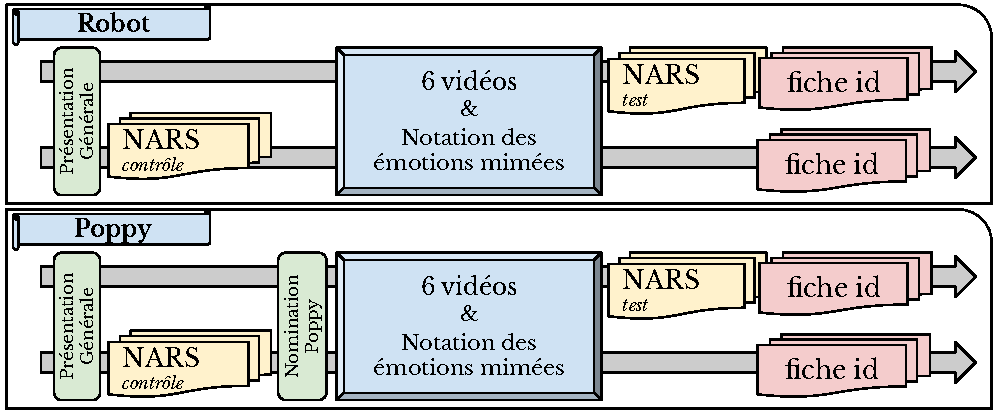
\includegraphics[width=\linewidth]{Figures/Desprez-proto-name_for_bot.pdf}
                    \caption{Protocole: \cro{un nom pour un robot}}\label{fig:proto-name_for_bot}
                \end{figure}
        \paragraph{Méthode} 
            Pour effectuer les passations, nous avons opté pour un formulaire en-ligne permettant ainsi une large diffusion ($N=106$), mais aussi par ce que le format vidéo imposait un support multimédia. 
            Les sujets étaient invités à visionner les vidéos (proposées dans un ordre aléatoire). Ces vidéos devaient être notées selon 6 critères émotionnels sur une échelle de -3 à +3 (de \gui{n'exprime absolument pas} à \gui{exprime parfaitement} telle émotion). Les 6 émotions sont le dégoût, la surprise, la joie, la colère, la tristesse et la peur.
            Deux conditions ont été créées, l’une où la question, portant sur la reconnaissance des émotions, était de la forme \gui{Poppy exprime\dots} et l’autre de la forme \gui{le Robot exprime\dots}. Parmi ces conditions, environ 20\prc des sujets effectuaient en premier lieu, la passation du \sht{NARS} pour constituer une ligne de base.
            \subparagraph{Matériel}
                \begin{figure}[!h]
                \begin{minipage}{0.375\linewidth}
                      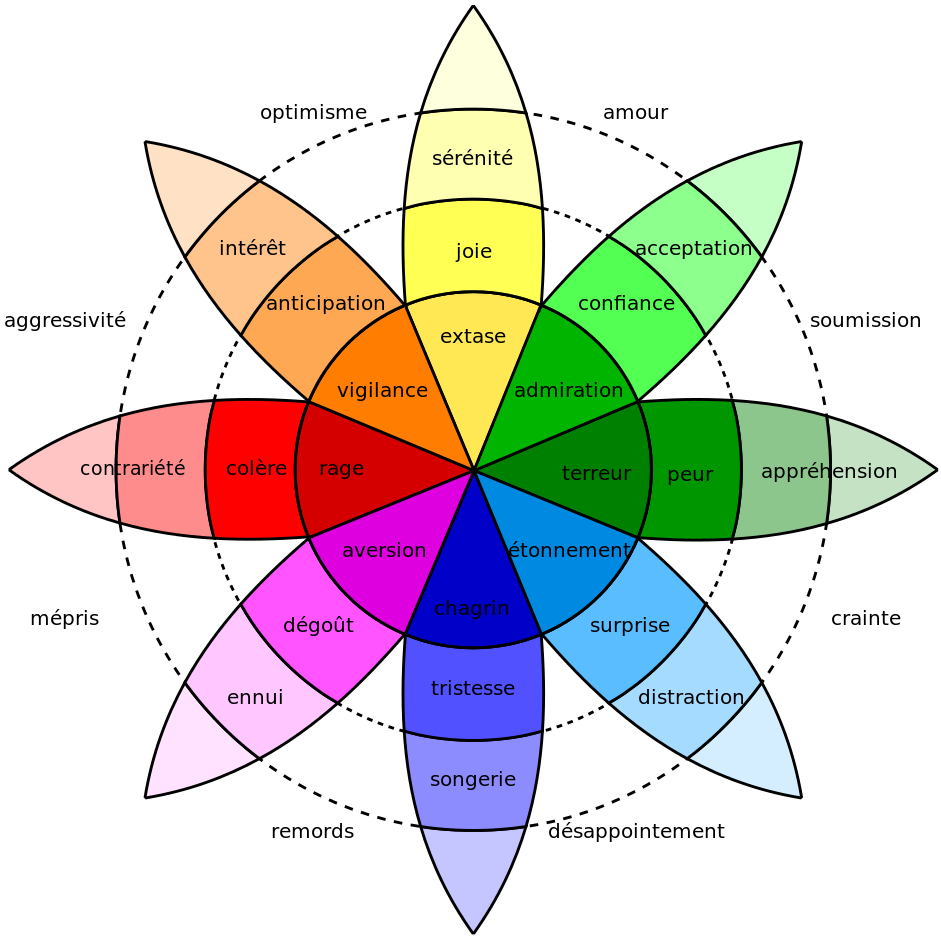
\includegraphics[width=\linewidth]{Figures/EmoModel.png}
                      \caption{Roue des émotions, Plutchik~\citeB{plutchik1991emotions}}\label{fig:EmoModel}
                \end{minipage}
                \hfill
                \begin{minipage}{0.6\linewidth}
                \myDefautStyle
                \subparagraph{Matériel vidéo}
                    Nous avons, dans certains cas, pu justifier clairement nos choix de mouvements, et dans d’autres nous avons dû nous baser essentiellement sur notre ressenti à l’aide de nos propres corps et en mimant les émotions nous mêmes ou encore en analysant certains cours de théâtre disponibles sur internet. Les archives de ces vidéos sont disponibles à une adresse \cro{non-répertoriée} permettant leur réutilisation future par d'autres équipes de recherche~\citeURL{TD-emo}.\newline\vfill
                \end{minipage}
                \end{figure}\par%
                \begin{itemize}\myItemStyle
                    \item    La tristesse: met en scène les mouvements classiques de la \gui{tragédie grecque} où l’homme se penche, prenant sa tête dans les mains pour pleurer.
                    \item    Le dégoût: l’idée était ici de mettre en scène l’apparition d’une odeur désagréable, le robot met une main sur son ventre, l’autre bouge légèrement devant son \gui{nez}.
                    \item    La joie: la difficulté d’exprimer la joie, sans l’aide du visage et avec une position des mains fixe (ouverte), était grande. L’idée était ici, d’avoir une sorte de danse de la victoire comme on peut l’observer dans certaines rencontres sportives.
                    \item    La colère: pour les mêmes raisons que la joie, cette expression était difficile à réaliser, pourtant le résultat est plutôt concluant.
                    \item    La surprise: certainement l’une des plus simple à réaliser, ici Poppy tourne la tête vers un objet qui le fait sursauter.
                    \item    La peur: est certainement la plus significative, car elle englobe l’émotion de la surprise tout en y ajoutant une notion de danger, caractérisée par la protection immédiate du corps (et principalement du visage) par les mains, puis par un moment d’attente et enfin de relâchement.
                \end{itemize}\par%
                Le score de reconnaissance:
                Pour chaque vidéo, on soustrait à la bonne réponse, la valeur moyenne des 5 mauvaises réponses. Exemple: vidéo colère: points colère - (moyenne (points: joie, tristesse, peur, dégoût, surprise).
                Puis on calcule la moyenne pour toutes les vidéos.\par%
                \vspace{-0.35cm}
                \begin{equation*}
                    Score=moyenne(V_T-(moyenne(V_n,V_n,V_n,V_n,V_n))
                \end{equation*}
                \newline\vspace{-1.75cm}
                \begin{multline*}\setstretch{1,0}\small
                    S=moy((V_1-(moy(V_2,V_3,V_4,V_5,V_6)));\\(V_2-(moy(V_1,V_3,V_4,V_5,V_6)));\dots\\\dots(V_6-(moy(V_1,V_2,V_3,V_4,V_5))))
                \end{multline*}
                \strut\hfill Score maximal: $S=5$ avec $V_n=0$ et $V_T=5$ \hfill Score minimal: $S=-5$ avec $V_n=5$ et $V_T=0$ \hfill\strut
        \paragraph{Résultats}
            \begin{figure}[!h]
            \begin{minipage}{0.425\linewidth}
                \centering
                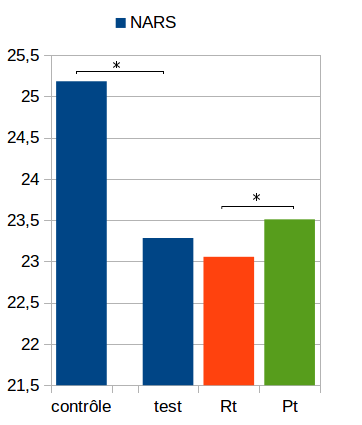
\includegraphics[width=.9\linewidth]{Figures/Desprez-nars-name_for_bot.png}
                \subcaption{Score obtenu au NARS}
                \label{fig:result-nars-name_for_bot}
            \end{minipage}
            \begin{minipage}{0.55\linewidth}
                \centering
                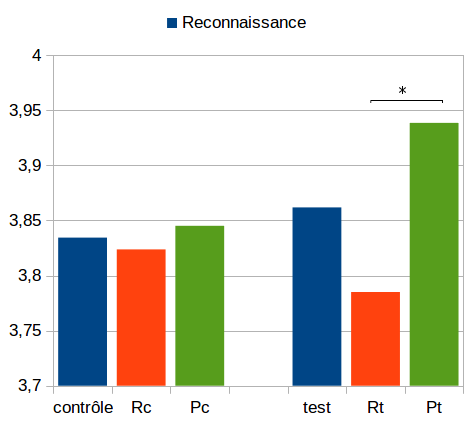
\includegraphics[width=.9\linewidth]{Figures/Desprez-BR-name_for_bot.png}
                \subcaption{Score de reconnaissance des émotions mimées}
                \label{fig:result-br-name_for_bot}
            \end{minipage}
            \caption{Résultats: \cro{un nom pour un robot}}
            \label{fig:result-name_for_bot}
            \end{figure}\par%
            Par rapport à nos hypothèses initiales, nous observons que, effectivement, nommer le robot par son prénom dans la formulation du questionnaire a un impact positif sur la capacité du sujet à déterminer la bonne émotion mimée dans les vidéos. En effet, sur la figure~\ref{fig:result-br-name_for_bot} nous voyons que dans la version \cro{test} (\sht{NARS} placé en aval) de la condition \cro{Poppy}, ici identifiée sous l'appellation \textit{Pt}, le score de reconnaissance est supérieur à 3,9~/~5, alors que dans le groupe \textit{Rt} ce score ne dépasse pas les 3,8~/~5. Bien que relativement faible, cette différence se révèle être significative par un test de Studente ($p=$). Notre 1\iere hypothèse est donc validée. \par%
            En revanche, pour la 2\nde, nous constatons sur la figure~\ref{fig:result-nars-name_for_bot}, un effet inverse à nos prévisions. En effet, les sujets de la condition \textit{Pt} obtiennent un score au \sht{NARS} plus élevé: 23,5 contre 23,05. Ici encore, bien que faible, cette différence se révèle être significative par un test de Studente ($p=$). Notre 2\nde hypothèse est donc \cro{inversement} validée, au sens où, la relation attendue fut observée mais avec des valeurs inverses.\par%
            Cette recherche, exploratoire, nous a permis d'observer deux autres effets inattendus: \Li la passation du \sht{NARS} en amont des vidéos biaise la reconnaissance. En effet, sur la figure~\ref{fig:result-br-name_for_bot}, nous constatons que l'effet observé en version \cro{test} (validant notre 1\iere hypothèse) disparaît totalement en version \cro{contrôle}. \ii le score initial au \sht{NARS} (groupe \cro{contrôle}, figure~\ref{fig:result-nars-name_for_bot}) est significativement plus élevé que pour le groupe ayant complété le questionnaire après le visionnage des vidéos: 25,2 contre 23,3 ($p=$).
        \paragraph{Conclusion}
            Ces résultats tendent à montrer que la nomination du robot est un facteur non négligeable, car elle impacte les perceptions de l'individu, et donc influencera l'interaction future. En effet, nommer le robot a permis une meilleure reconnaissance des sets de 6 émotions humaines qu'il mimait en vidéo. De plus, nous constatons que visionner ces vidéos diminue le score au \sht{NARS} comme si celles-ci avaient un pouvoir de sensibilisation, ou d'accommodation des sujets à la robotique. En revanche, si nous nous focalisons uniquement sur les résultats post-vidéos, on note que c'est dans la condition où le robot est nommé que le score est le plus élevé. Les raisons de cette diminution plus faible dans cette condition reste une question ouverte, tout comme les raisons pour lesquelles le \sht{NARS} placé en amont des vidéos biaise la reconnaissance.
    \subsection{Synthèse}
        Ainsi, cette double approche: longitudinale et ponctuelle, nous a permis d'enrichir nos connaissances sur les facteurs facilitant l'acceptabilité de la robotique. 
        Tout d'abord, \sht{EURO382} nous a permis de constater une évolution positive dans la perception de la robotique entre 2012 et 2017. Mais également de constater que les activités robotiques pratiquées par les élèves \tiret{et les différentes caractéristiques de celles-ci} influençaient cette dimension.
        Pour autant, nous n'avons pas été en mesure d'isoler, à posteriori, quelles caractéristiques mises en place par l'enseignant, avaient pu être déterminantes dans l'impact global observé. 
        Dans la seconde expérience présentée, nous avons pu mettre en lumière que ces caractéristiques déterminantes pouvaient se situer sur des éléments semblant insignifiants telle que la nomination de l'objet robotique qui, ici, a montré son impact sur la perception de l'objet en lui-même et des robots en général.